\section{Laplaceovo rozdělení}

Pro Laplaceovo rozdělení je hustota pravděpodobnosti
\begin{equation}
	p_{\theta}(x)  = \frac{1}{2\sigma} e^{ -\frac{| x-\mu |}{\sigma}  } 
\end{equation}

což znamená, že parametrem rozdělení pro nás bude $\theta = (\mu,\sigma)$, tedy $\Theta = \mathbb{R} \times \mathbb{R}^+ $. Pro $\alpha > 0 $ máme 

\begin{equation}
		\intpa	= \frac{(2\sigma)^{-\alpha}}{(1+\alpha)}. 
\end{equation}

Minimální Rényiho odhad pak můžeme pro $\alpha>0$ psát jako

\begin{equation}
	\theta_{\alpha,n} = \amtiT (2\sigma)^{-\frac{\alpha}{1+\alpha}} \frac{1}{n} \sum_{i=1}^n e^{-\alpha\frac{| x_i-\mu |}{\sigma}}. 
\end{equation}

Influenční funkce pro tento odhad je tvaru 
\begin{equation}
	\mathrm{IF}(x;T_{\alpha},\sigma) = (1 + \alpha)^2 \left( e^{-\frac{\alpha|x|}{\sigma}}\right) \left(-\sigma + (1 + \alpha)|x|\right)	
\end{equation}
a
\begin{equation}
	\mathrm{IF}(x;T_{\alpha},\mu) =(1+\alpha )^{\frac{3}{2}} e^{-\frac{\alpha}{2} (x-\mu )^2}  (x-\mu )
\end{equation}

\begin{figure}[htb]
  \centering
    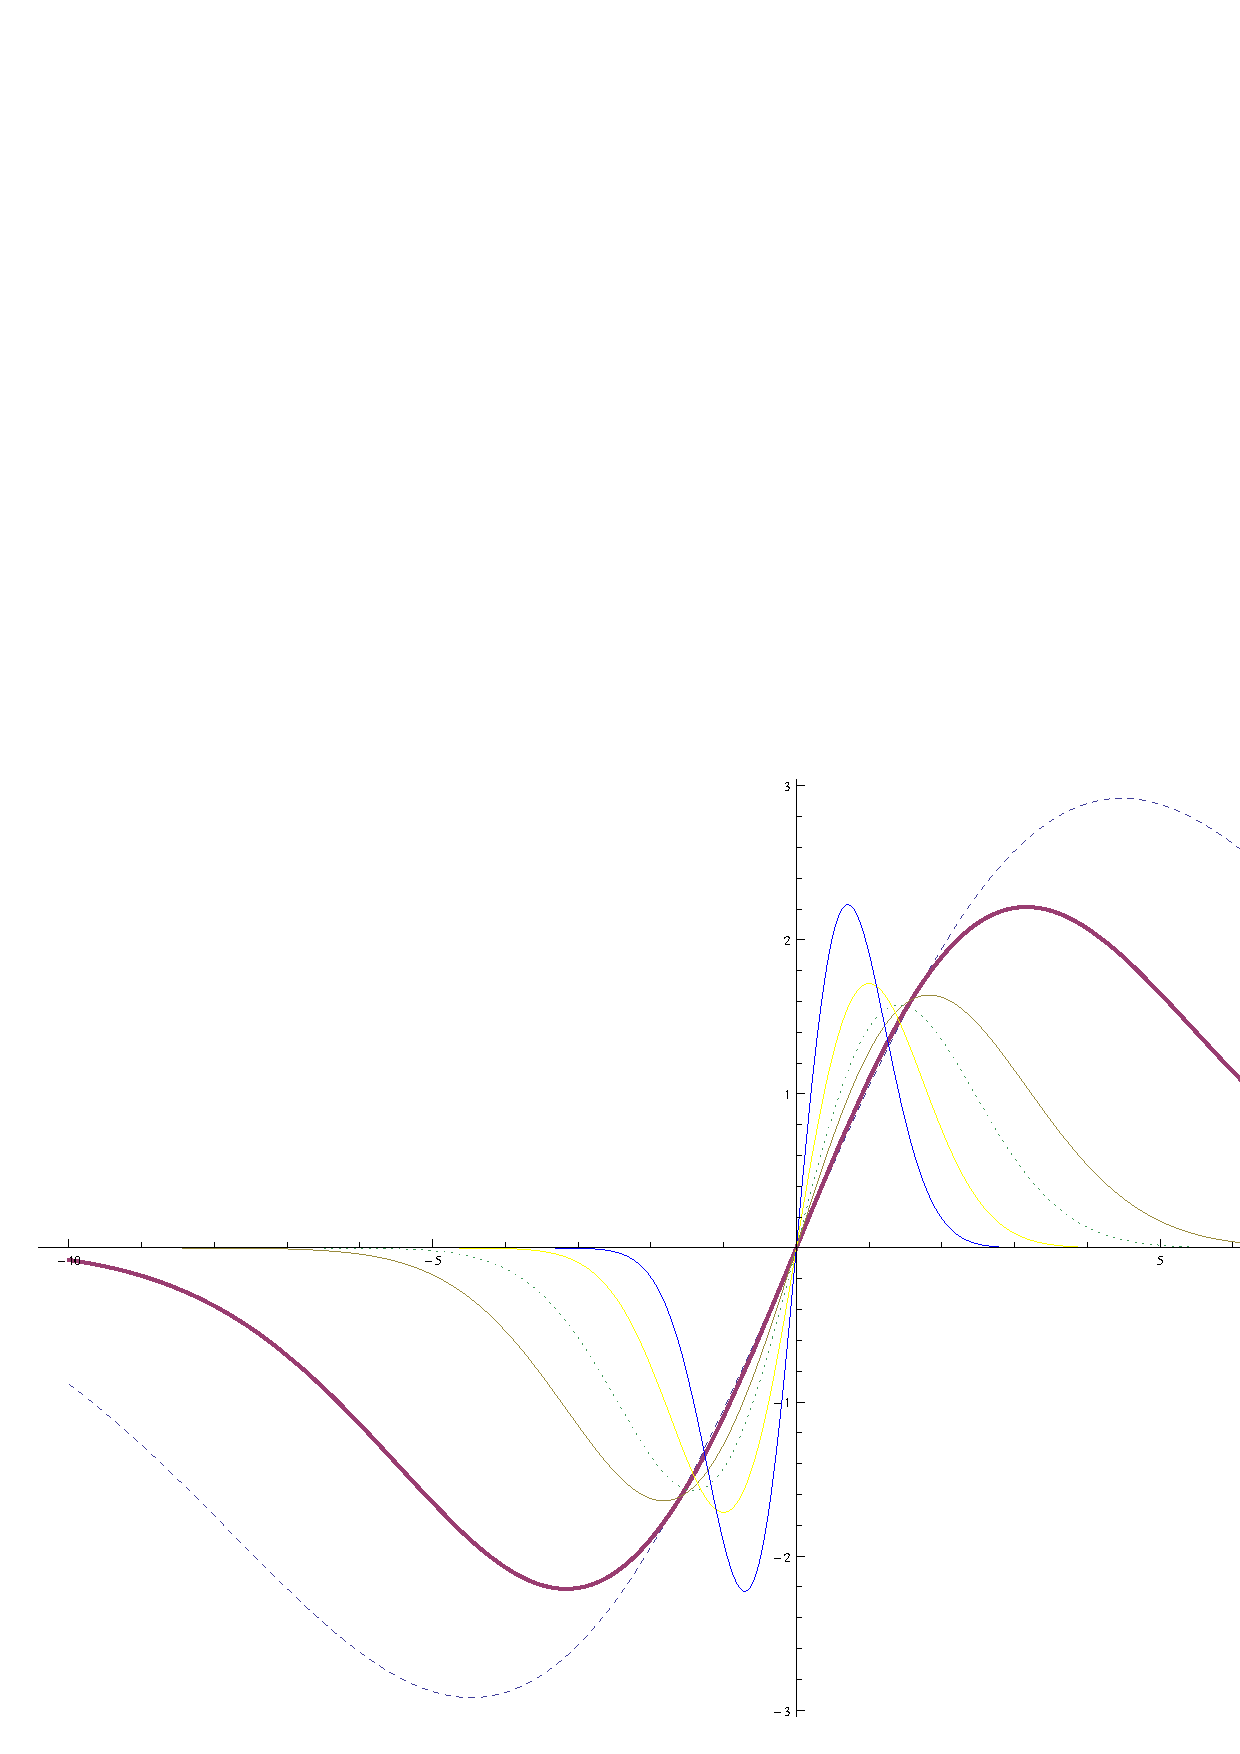
\includegraphics[scale=0.30]{IF-Laplace-mu.png}
          \caption{Influenční funkce pro parametr polohy}
    \label{fig:IF-Laplace-mu}
\end{figure}

\begin{figure}[htb]
  \centering
    \includegraphics[scale=0.30]{IF-Laplace-sigma.png}
          \caption{Influenční funkce pro parametr rozptylu}
    \label{fig:IF-Laplace-sigma}
\end{figure}


%
%\begin{eqnarray}
%	\intpa & = & \int_{-\infty }^{\infty } \left( {\frac{1}{2\sigma} \exp{ \left[ -\frac{|x -\mu |}{\sigma } \right] }} \right) ^{1 + \alpha} \, \mathrm{d}x \nonumber\\
%	 & = & \int_{-\infty }^{\mu } {\frac{1}{ (2\sigma)^{ 1 + \alpha}} \exp{ \left[ \frac{(1 + \alpha )(x -\mu )}{\sigma } \right] }} \, \mathrm{d}x \nonumber\\
%	 & + & \int_{\mu }^{\infty } {\frac{1}{ (2\sigma)^{ 1 + \alpha}} \exp{ \left[ -\frac{(1 + \alpha )(x -\mu )}{\sigma } \right] }} \, \mathrm{d}x \nonumber
%\end{eqnarray} 
%
%substituujeme $ y = \frac{(1+\alpha)(x-\mu)}{\sigma} $, tedy $\mathrm{d}y = \frac{1+\alpha}{\sigma}\mathrm{d}x $, pak
%
%\begin{eqnarray}
%	\intpa & = & \frac{1}{ (2\sigma)^{ 1 + \alpha}} \frac{\sigma}{1+\alpha} \left( 
%	\int_{-\infty }^{0 } {\exp{ \left[ y \right] }} \, \mathrm{d}x + 
%	\int_{0 }^{\infty } {\exp{ \left[ -y \right] }} \, \mathrm{d}x \right) \nonumber\\
%	& = & \frac{1}{ (2\sigma)^{ 1 + \alpha}} \frac{\sigma}{1+\alpha} \cdot 2  \nonumber\\
%	& = & \frac{(2\sigma)^{-\alpha}}{(1+\alpha)} 
%\end{eqnarray}
%tedy 
%\begin{eqnarray}
%	\theta_{\alpha,n} &= &\amtiT \left( \frac{(2\sigma)^{-\alpha}}{(1+\alpha)}  \right)^{-\frac{\alpha}{1+\alpha}} \frac{1}{n} \sum_{i=1}^n \frac{1}{(2\sigma)^{\alpha}} \exp \left[-\alpha\frac{|x_i-\mu|}{\sigma} \right] \nonumber\\
%	&=& \amtiT (2\sigma)^{-\frac{\alpha}{1+\alpha}} \frac{1}{n} \sum_{i=1}^n \exp \left[-\alpha\frac{|x_i-\mu|}{\sigma} \right]
%\end{eqnarray}



